%%%
%
% $Autor: Wings $
% $Datum: 2021-05-14 $
% $Pfad: GitLab/MLEdgeComputer $
% $Dateiname: AppADPS9960
% $Version: 4620 $
%
% !TeX spellcheck = de_DE/GB
% !TeX program = pdflatex
% !BIB program = biber/bibtex
% !TeX encoding = utf8
%
%%%



\chapter{Application of the Color Sensor with OLED Display}

The color detection machine utilizes an Arduino Nano 33 BLE Sense with an APDS-9960 sensor for reliable recognition of red, green, and blue colors, making it suitable for various industrial automation processes. Every 750 ms, the machine reads the color of an object and displays the result on an OLED screen. Before each color reading, the proximity sensor checks if an object is close to the sensor, if so, the white LED activates to improve sensor accuracy in low-light conditions.

\section{Manual}
The color detection machine consists of the Arduino Nano 33 BLE Sense and a 1.30" IIC OLED display, which need to be connected according to the circuit diagram in Figure \ref{fig:OLEDCircuit}.

\begin{center}
    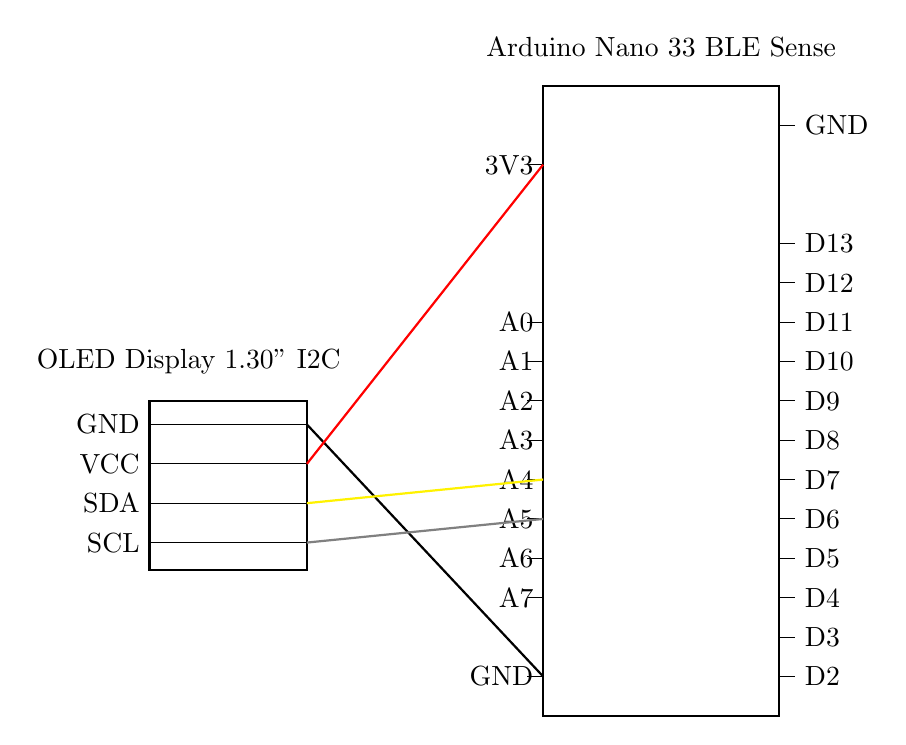
\begin{tikzpicture}
        % Arduino Nano 33 BLE Sense
        \node at (5.5, 8.5) {Arduino Nano 33 BLE Sense}; % Label above the Arduino
        \draw[thick] (4, 0) rectangle (7, 8);
        
        % Left side pins
        \foreach \i/\label in {0.5/GND, 1.5/A7, 2/A6, 2.5/A5, 3/A4, 3.5/A3, 4/A2, 4.5/A1, 5/A0, 7/3V3} {
            \draw (3.8, \i) -- (4, \i) node[left] {\label};
        }
        
        % Right side pins
        \foreach \i/\label in {0.5/D2, 1/D3, 1.5/D4, 2/D5, 2.5/D6, 3/D7, 3.5/D8, 4/D9, 4.5/D10, 5/D11, 5.5/D12, 6/D13, 7.5/GND} {
            \draw (7, \i) -- (7.2, \i) node[right] {\label};
        }
        
        % OLED Display
        \node at (-0.5, 4.5) {OLED Display 1.30'' I2C}; % Label above the OLED display
        \draw[thick] (-1, 1.85) rectangle (1, 4);
        
        % OLED pin labels on the left, pins on the right
        \foreach \i/\label in {2.2/SCL, 2.7/SDA, 3.2/VCC, 3.7/GND} {
            \draw (-1, \i) node[left] {\label} -- (1, \i);
        }
        
        % Connections
        \draw[thick, black] (4, 0.5) -- (1, 3.7); % GND to GND
        \draw[thick, red] (4, 7) -- (1, 3.2); % 3V3 to VCC
        \draw[thick, yellow] (4, 3) -- (1, 2.7); % A4 to SDA
        \draw[thick, gray] (4, 2.5) -- (1, 2.2); % A5 to SCL
        
    \end{tikzpicture}
    \captionof{figure}{Circuit diagram for connecting the Arduino Nano 33 BLE Sense with a 1.30” IIC OLED display.}
    \label{fig:OLEDCircuit}
\end{center}

Use a laptop or computer to open the \texttt{ApplicationAPDS9960} code in the Arduino IDE. Before uploading the code, enter the \texttt{maxRed}, \texttt{maxGreen}, and \texttt{maxBlue} calibration values to ensure accurate color detection by the machine.

Once the Arduino is programmed, the color detection machine can start. Place an object approximately one centimeter in front of the APDS-9960 sensor on the Arduino. The OLED display will show important instructions and display detected colors. Each time an object is removed and replaced, the sensor will read the color in its usual interval. Ensure proper lighting, and calibrate the sensor under the same conditions in which it will operate.

\section{Code Explanation}

The following section provides an explanation of the application code:

\smallskip

The first part of the code initializes the Arduino Nano 33 BLE Sense with the APDS-9960 sensor and the 1.30" IIC OLED display. It includes pre-determined calibration values for red, green, and blue (\texttt{maxRed}, \texttt{maxGreen}, \texttt{maxBlue}) as integer values. In the \texttt{setup()} function, it starts serial communication, sets the LED pin as an output, and initializes the APDS-9960 sensor, printing an error message if the initialization fails. It also sets up the OLED display to show an "INITIALIZING!" message. Afterward, the LED blinks three times to indicate that the setup is complete, and the display is cleared.

{
	\captionof{code}{Application of the sensor APDS9960: Setup}\label{AppAPDS9960Header}
	\ArduinoExternal{firstline=1,lastline=52}{../../Code/Nano33BLESense/APDS9960/ApplicationAPDS9960/ApplicationAPDS9960.ino}
}


In the following \texttt{loop()} function, the code displays a "READY" message on the OLED display and then sets a timeout of 1000 ms to wait for color data to become available, decrementing the timeout in steps of 5 ms. If color data is not available within the timeout, a "Color measurement timeout" message is printed in the serial monitor, and the function returns. The code then resets the timeout to 1000 ms and similarly waits for proximity data. If proximity data does not become available within the timeout, a "Proximity measurement timeout" message is printed, and the function returns.

{
	\captionof{code}{Application of the sensor APDS9960: Loop}\label{AppAPDS9960Loop}
	\ArduinoExternal{firstline=53,lastline=81}{../../Code/Nano33BLESense/APDS9960/ApplicationAPDS9960/ApplicationAPDS9960.ino}
}


In the next section of the \texttt{loop()} function, the code reads the proximity value using \texttt{APDS.readProximity()}. If a valid proximity value is detected, it prints the proximity value to the serial monitor. If the proximity value is below a specified threshold (indicating an object is close), the OLED display is cleared, and the LED is turned on as a visual indication. To capture accurate color data, all LEDs are turned on to emit white light, and multiple color readings are averaged.

The red, green, and blue color values are then mapped to a 0-255 range using predefined calibration values (\texttt{maxRed}, \texttt{maxGreen}, \texttt{maxBlue}) and are constrained within the 0-255 range. The dominant color is determined based on the highest value among red, green, and blue, and the result is displayed on the OLED. If no object is detected within the proximity threshold, a message prompts the user to hold an object near the sensor or change its position.

If the proximity reading fails, an error message is displayed on the OLED. After processing, the code turns off the LED and resets the RGB LEDs to an off state.

{
	\captionof{code}{Application of the sensor APDS9960: Main function}\label{AppAPDS9960Main}
	\ArduinoExternal{firstline=83,lastline=174}{../../Code/Nano33BLESense/APDS9960/ApplicationAPDS9960/ApplicationAPDS9960.ino}
}


\section{Application Test}

The color recognition machine reliably identifies the colors red, green, and blue from the standardized color chart. After calibration, it can also recognize other colors like light blue, yellow-green, or orange as red, green, and blue. This flexibility ensures that objects do not need to be perfectly red, green, or blue to be detected. Activating the white LED when an object approaches proves to be very practical, as it serves as a feedback mechanism alongside the OLED display, indicating to the user that color recognition is now in progress.

\section{Improvement Suggestions}

A key improvement would be to integrate the color recognition machine into a stable, standalone setup, so it does not need to be handheld, allowing objects to be fixed in place in front of the sensor. This would eliminate potential issues like hand movement artifacts during detection.

Another enhancement would be to equip the device with a battery, enabling portable, laptop-free operation. To conserve battery life, the white LED is deliberately programmed to illuminate only during color measurement. 

In an industrial application, adequate lighting should be ensured, potentially by adding external lighting that could be integrated into the code or kept continuously on. For use in dusty or humid environments, a thin protective cover over the sensor could prevent damage or contamination, allowing for easy cleaning or replacement as needed.

